\documentclass{sigchi}

% Use this command to override the default ACM copyright statement (e.g. for preprints). 
% Consult the conference website for the camera-ready copyright statement.


% Arabic page numbers for submission. 
% Remove this line to eliminate page numbers for the camera ready copy
%\pagenumbering{arabic}



\usepackage{balance}  % to better equalize the last page
\usepackage{graphics} % for EPS, load graphicx instead
\usepackage{times}    % comment if you want LaTeX's default font
\usepackage{url}      % llt: nicely formatted URLs
\usepackage{graphicx}
\usepackage{caption}
\usepackage{subcaption}
\usepackage{array}

% llt: Define a global style for URLs, rather that the default one
\makeatletter
\def\url@leostyle{%
  \@ifundefined{selectfont}{\def\UrlFont{\sf}}{\def\UrlFont{\small\bf\ttfamily}}}
\makeatother
\urlstyle{leo}


% To make various LaTeX processors do the right thing with page size.
\def\pprw{8.5in}
\def\pprh{11in}
\special{papersize=\pprw,\pprh}
\setlength{\paperwidth}{\pprw}
\setlength{\paperheight}{\pprh}
\setlength{\pdfpagewidth}{\pprw}
\setlength{\pdfpageheight}{\pprh}

% Make sure hyperref comes last of your loaded packages, 
% to give it a fighting chance of not being over-written, 
% since its job is to redefine many LaTeX commands.
%\usepackage[pdftex]{hyperref}
%\hypersetup{
%pdftitle={L@S 2014 Work-in-Progress Format},
%pdfauthor={LaTeX},
%pdfkeywords={SIGCHI, proceedings, archival format},
%bookmarksnumbered,
%pdfstartview={FitH},
%colorlinks,
%citecolor=black,
%filecolor=black,
%linkcolor=black,
%urlcolor=black,
%breaklinks=true,
%}

% create a shortcut to typeset table headings
\newcommand\tabhead[1]{\small\textbf{#1}}

\begin{document}

\title{Exploring Regression}


\maketitle

\large

\section{Gradient Descent}

We implemented a function
\[\textsc{Gradient-Descent($f, f', g, \lambda, c$)}\]
to compute the minimum of a scalar function of a vector argument. In addition to the objective function $f$, the user can specify the gradient function $f'$, the initial guess $g$, the step size $\lambda$, and the convergence criterion $c$.

The choice of initial guess, step size, and convergence criterion can have a drastic effect on the resulting solution.

Choosing an initial guess that is close to a solution will make \textsc{Gradient-Descent} converge more quickly. Choosing an initial guess that is on a downward slope into a particular solution will probably make the ultimate result be that solution. Therefore, \textsc{Gradient-Descent} will return a better solution if the initial guess is on a downward slope into a global maximum, and a worse solution if the starting guess is on a downward slope into a mediocre local maximum.

A smaller step size will make \textsc{Gradient-Descent} converge more slowly. However, if the initial step size is too large, the algorithm could oscillate around the minimum and never converge on the solution. Worse, it could oscillate back and forth in an increasing manner and suffer an exponential blowup \emph{away} from any minima.

With a smaller convergence criterion \textsc{Gradient-Descent} will return a solution which is closer to the actual minimum. However, it will require more iterations. A small convergence criterion combined with a large step size could create the risk that the algorithm will diverge.

The gradient function $f'$ will use central differences to estimate the gradient at any given point. Consider the quartic bowl $f(x_1, x_2) = x_1^4 + x_2^4$. Figure 1 shows the gradients produced by our $f'$ compared to the actual gradients. We can see that for a smooth function like the quartic bowl, our gradient estimation will be very close to the actual gradient.

\begin{figure}
\def\arraystretch{1.4}

\begin{center}
\begin{tabular}{| c | c | c |}
\hline
Point & Estimated Gradient& Actual Gradient\\
\hline
$(2, 0)$& $(32.02, 0)$ & $(32, 0)$ \\
\hline
$(3, 5)$& $(108.03, 500.05)$ &$(108, 500)$\\
\hline
$(-4, 8)$&$(-256.04, 2048.08)$ & $(-256, 2048)$\\
\hline
\end{tabular}
\end{center}
\caption{Performance of our gradient estimator on the function $f(x_1, x_2) = x_1^4 + x_2^4$.}
\end{figure}


Consider the Python function \textsc{Fmin-Bfgs}. We ran both optimization functions with the same parameters and compared the number of times that $f$ was evaluated. The results of our experiments are shown in Figure 2.

\begin{figure}
\def\arraystretch{1.4}

\begin{center}
\begin{tabular}{| c | c | c |}
\hline
$f$ & \textsc{Gradient-Descent} & \textsc{Fmin-Bfgs}\\
\hline
$x_1^2 + x_2^2$ & 1680 & 16 \\
\hline
$x^4 - x^3 - x^2 + x$ & 388 & 57\\
\hline
\end{tabular}
\end{center}
\caption{Table of number of function calls. The initial guess was $(5, 5)$ for the first row and $-5$ for the second.}
\end{figure}

Clearly \textsc{Gradient-Descent} takes far more iterations to converge than the more sophisticated optimizer. One possible improvement to \textsc{Gradient-Descent} which could drastically reduce the number of iterations would be to vary the step size.


\section{Linear Basis Function Regression}

Consider the class of regression models consisting of a linear combination of polynomial basis functions. The goal is to determine a function
\[f(x) = w_0 + w_1x + w_2x^2 + \hdots + w_Mx^M,\]
such that the sum of square errors (SSE) of the actual data is minimized. We can solve this problem by using \textsc{Gradient-Descent} to solve for the value of $w$ that minimizes the SSE.

Consider the data set shown in Bishop Figure 1.4, and the curves shown for various values of $M$. Using \textsc{Gradient-Descent} to minimize SSE, we are able to replicate these curves very closely by carefully choosing our parameters. For $M = 0$ and $M = 1$, the curves produced by \textsc{Gradient-Descent} are almost identical to those in the original plots, even when given an initial guess which is very far from the solution. These plots are shown in Figure 3.

\begin{figure}[!t]
\centering
\begin{subfigure}[b]{2.25in}
	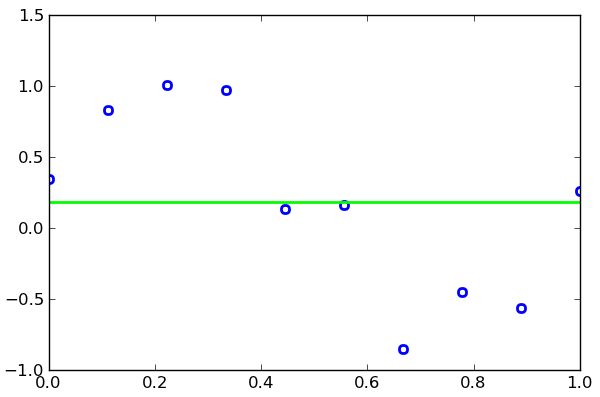
\includegraphics[width = 2.25in]{m0.png}
	\caption{$M = 0$}
\end{subfigure}
\begin{subfigure}[b]{2.25in}
	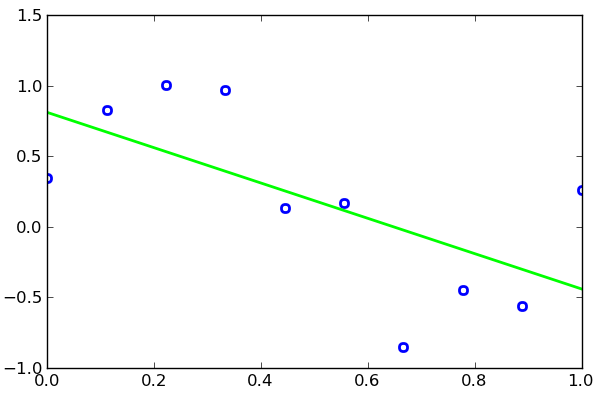
\includegraphics[width = 2.25in]{m1.png}
	\caption{$M = 1$}
\end{subfigure}
\caption{Results of using \textsc{Gradient-Descent} to minimize the SSE with various values of $M$.}
\end{figure}

However, once we fit the data with $M = 3$, \textsc{Gradient-Descent} begins to show its weaknesses. If the initial guess is not reasonably close to the desired solution, \textsc{Gradient-Descent} is unable to converge upon the answer. If the convergence criterion is too large, then the function terminates at a suboptimal point. However, if the convergence criterion is too small, the function requires prohibitively many iterations in order to converge.

If our initial guess for \textsc{Gradient-Descent} is close to the desired weight vector, then it will converge quickly upon the correct weight vector. Figure 4 shows the results of two calls to \textsc{Gradient-Descent} when $M = 3$. Plot (a) shows the result when the initial vector is $(0, 0, 0, 0)$, and plot (b) shows when the initial weight vector is $(20, 20, -20, 20)$ (the solution is roughly $(0, 8, -25, 17)$). We can see that the curve in plot (b) very closely resembles the curve in the original graph.

\begin{figure}[!t]
\centering
\begin{subfigure}[b]{2.25in}
	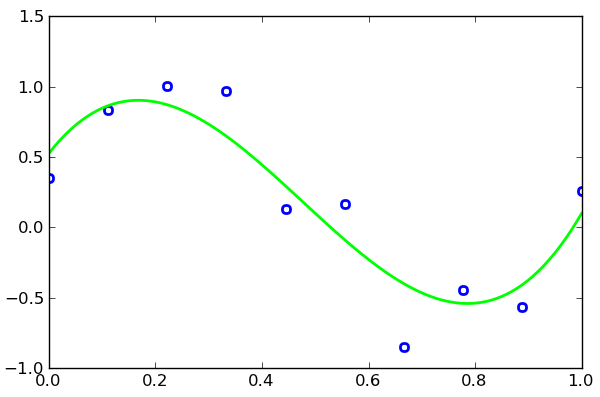
\includegraphics[width = 2.25in]{m3_0.png}
	\caption{$M = 3, g = (0, 0, 0, 0)$}
\end{subfigure}
\begin{subfigure}[b]{2.25in}
	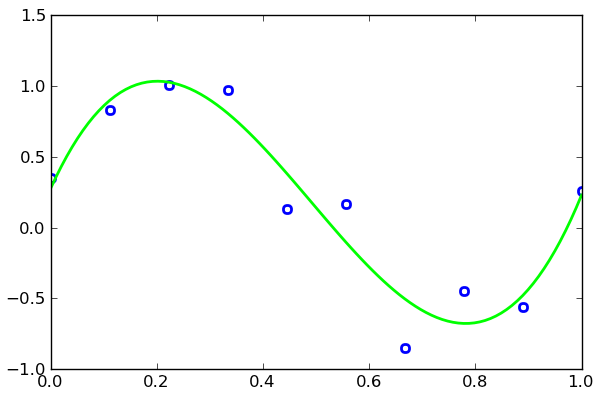
\includegraphics[width = 2.25in]{m3_1.png}
	\caption{$M = 3, g = (20, 20, -20, 20)$}
\end{subfigure}
\caption{Results of using \textsc{Gradient-Descent} to minimize the SSE with $M = 3$, with a bad initial guess and an initial guess closer to the optimal solution.}
\end{figure}

\textsc{Fmin-Bfgs} was able to quickly converge on the correct weight vector for $M = 0$, $M = 1$, and $M = 3$.

\section{Ridge Regression}

In the case where we have a lot of features but not much data, it can be beneficial to reduce the variance of the produced estimates. One possible way to do this is with ridge regression. In ridge regression, we favor smaller weights by quadratically punishing proportional to the magnitude of the weight vector.

We implemented this algorithm as
\[\textsc{Ridge-Regression($x, y, M, \lambda$)}.\]
We can use this algorithm to find the weight vectors for the Bishop data set from the previous section. With $\lambda = 0$, \textsc{Ridge-Regression} found solutions very similar to those provided by Bishop. However, even with small non-zero values of $\lambda$, the curves produced by \textsc{Ridge-Regression} changed significantly.

\begin{figure*}[!t]
\centering
\begin{tabular}{c c c}
\begin{subfigure}[b]{2.25in}
	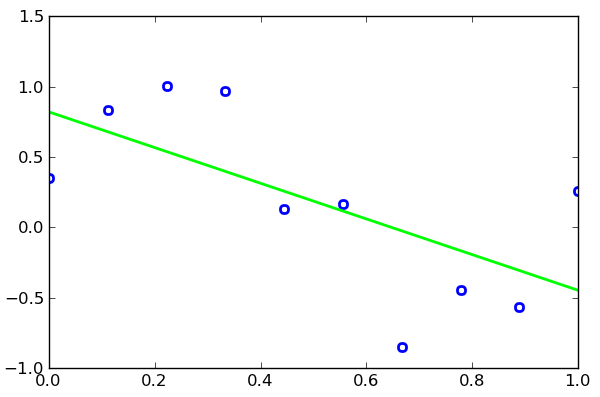
\includegraphics[width = 2.25in]{3-1-0.png}
	\caption{$M = 1$, $\lambda = 0$}
\end{subfigure} &

\begin{subfigure}[b]{2.25in}
	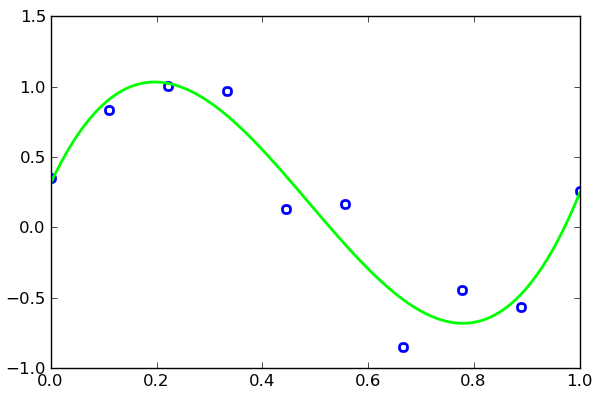
\includegraphics[width = 2.25in]{3-3-0.png}
	\caption{$M = 3$, $\lambda = 0$}
\end{subfigure} &

\begin{subfigure}[b]{2.25in}
	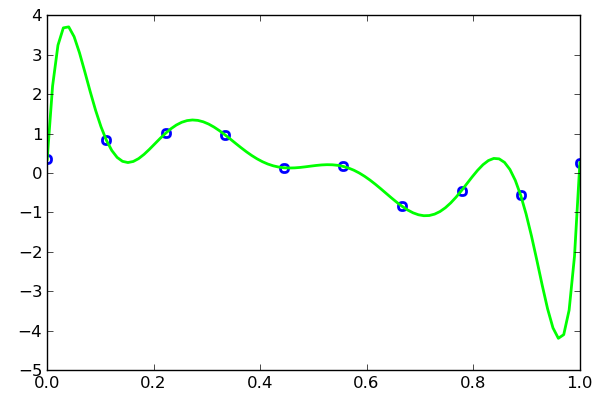
\includegraphics[width = 2.25in]{3-9-0.png}
	\caption{$M = 9$, $\lambda = 0$}
\end{subfigure} \\


\begin{subfigure}[b]{2.25in}
	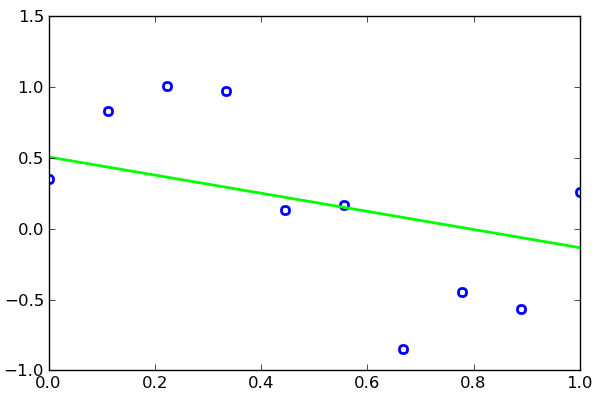
\includegraphics[width = 2.25in]{3-1-1.png}
	\caption{$M = 1$, $\lambda = 1$}
\end{subfigure} &

\begin{subfigure}[b]{2.25in}
	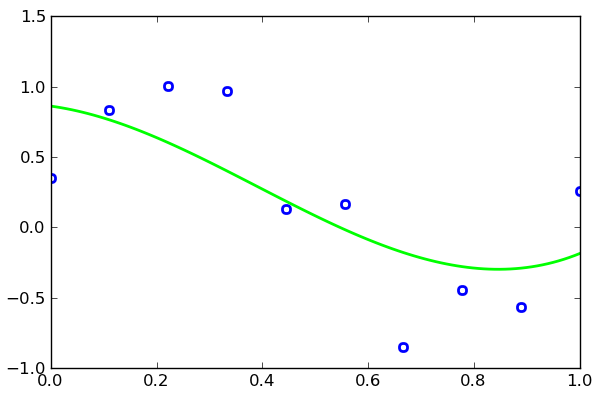
\includegraphics[width = 2.25in]{3-3-01.png}
	\caption{$M = 3$, $\lambda = 0.01$}
\end{subfigure} &

\begin{subfigure}[b]{2.25in}
	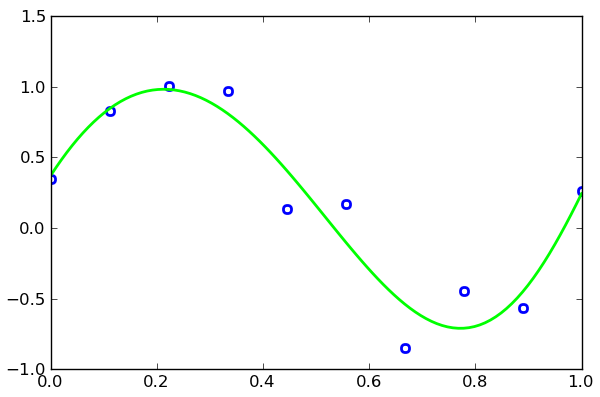
\includegraphics[width = 2.25in]{3-9-0001.png}
	\caption{$M = 9$, $\lambda = 0.0001$}
\end{subfigure} \\
\end{tabular}
\caption{Curves produced by \textsc{Ridge-Regression} for varying values of $M$ and $\lambda$. Columns contain the same $M$ value. The top row has $\lambda = 0$, while the bottom row has nonzero $\lambda$ values.}
\end{figure*}

Shown in Figure 5 are the curves produced by \textsc{Ridge-Regression} for various values of $M$ and $\lambda$. The first column shows $M = 1$, the second column $M = 3$, and the third column $M = 9$. The plots in the top row all have $\lambda = 0$, while the plots in the bottom row have $\lambda$ set to some small non-zero value (which varies across the plots).

The first observation we make is that the larger the value of $M$, the smaller $\lambda$ needed to be in order to make a noticeable difference on the curve. This is very intuitive, because for larger $M$ $w$ is a higher dimensional vector and thus has greater magnitude.

Next, we notice that the curves with non-zero $\lambda$ values are very similar to the curves for lower $M$ values with $\lambda = 0$. In particular, plot (e) resembles plot (a), and plot (f) is very similar to plot (b). Thus, as we increase the value of $\lambda$, we push the curves towards solutions with lower values of $M$.


\subsection{Model Selection}

Next, we want to use \textsc{Ridge-Regression} in order to implement model selection. To do this, we will first use \textsc{Ridge-Regression}  (for some $M$ and $\lambda$) to compute the weight vector using a set of training data. Next, we will test the performance of this weight vector against a set of validation data. We want to choose the values of $M$ and $\lambda$ which minimize the SSE on the validation data.

We performed model selection using two different sets of training data, which we will refer to as ``Regression Data A'' and ``Regression Data B''. The following sections describe our findings.

\subsubsection{Regression Data A}

For any given value of $M$, it is possible to compute the optimal value of $\lambda$ by computing the value of $\lambda$ which minimizes the SSE on the validation data. We computed this value using \textsc{Fmin-Bfgs}. Figure 6 shows a graph of validation SSE versus $\lambda$ for $M = 4$.

\begin{figure}[!t]
\centering
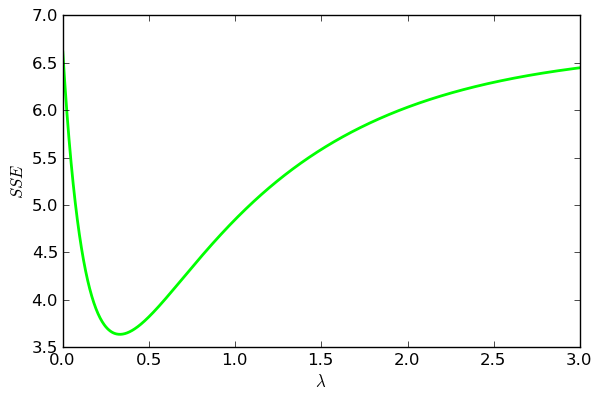
\includegraphics[width=3in]{min_lam.png}
\caption{SSE of the validation data plotted against the value of $\lambda$ used in \textsc{Ridge-Regression} on Regression Data A. For our model, we want to choose the value of $\lambda$ which minimizes SSE.}
\end{figure}

Sometimes, the optimal value of $\lambda$ turns out to be negative. However, a negative value of $\lambda$ corresponds to rewarding large weights, which must be undesirable because it encourages overfitting. Thus, whenever the optimal value of $\lambda$ is negative, we choose $\lambda = 0$.

The table in Figure 7 displays values of $M$ along with their corresponding optimal values of $\lambda$, and the resulting SSE of the validation data.

\begin{figure}[!]
\centering
\def\arraystretch{1.4}

\newcolumntype{C}[1]{>{\centering\let\newline\\\arraybackslash\hspace{0pt}}m{#1}}

\begin{tabular}{| C{0.75in} | C{0.75in} | C{0.75in} |}

\hline
$M$ & $\lambda$ & SSE\\
\hline
1 & 0 & 1.958\\
\hline
2 & 0 & 2.297\\
\hline
3 & 0 & 3.674\\
\hline
4 & 0.331 & 3.637\\
\hline
5 & 0.121 & 3.976\\
\hline
\end{tabular}
\caption{Optimal values of $\lambda$ when trained on Regression Data A for various values of $M$, along with the resulting SSE of the validation data.}
\end{figure}

We can see that the values which minimizes the SSE on the validation data are $M = 1$ and $\lambda = 0$, so we choose these for our model. The resulting curves are shown in Figure 8 against the training and validation data.

While it is slightly unsatisfying that we end up choosing a simple linear model, we can clearly see that the data (particularly the validation set) fits closely to a line. The fact that the validation data seems to have a slightly steeper slope than the training data justifies why the optimal value for $\lambda$ with $M = 1$ was actually negative.

\begin{figure}[!t]
\centering
\begin{tabular}{c}

\begin{subfigure}[b]{2.25in}
	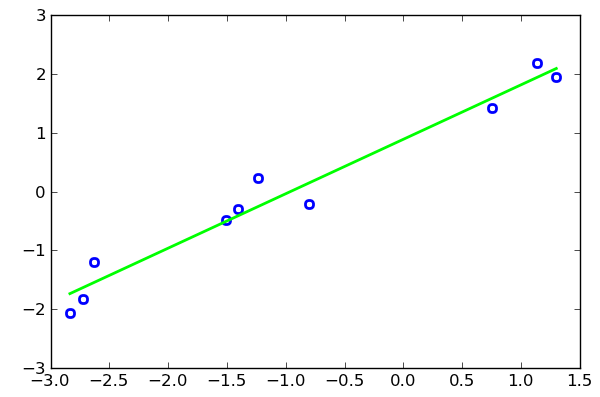
\includegraphics[width = 2.25in]{A-1-0.png}
	\caption{Training data, $M = 1$, $\lambda = 0$}
\end{subfigure} \\

\begin{subfigure}[b]{2.25in}
	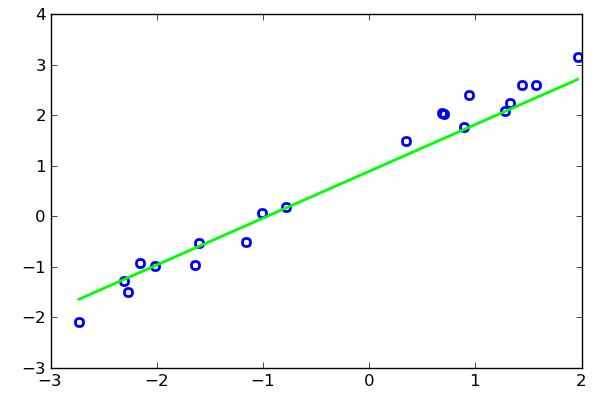
\includegraphics[width = 2.25in]{AV-1-0.png}
	\caption{Validation data, $M = 1$, $\lambda = 0$}
\end{subfigure} \\

\end{tabular}

\caption{The best fit for \textsc{Ridge-Regression} using Regression Data A as training data.}
\end{figure}

\subsubsection{Regression Data B}

Next we use the same process on Regression Data B. The most noticeable difference about the Regression Data B is the presence of an outlier. Because we are trying to minimize SSE, the outlier will always have a large impact on the chosen weights. Thus, we do not expect to be able to find values of $M$ and $\lambda$ such that the curve fits the validation data very well.

\begin{figure}
\centering
\def\arraystretch{1.4}

\newcolumntype{C}[1]{>{\centering\let\newline\\\arraybackslash\hspace{0pt}}m{#1}}

\begin{tabular}{| C{0.75in} | C{0.75in} | C{0.75in} |}

\hline
$M$ & $\lambda$ & SSE\\
\hline
1 & 0 & 35.106\\
\hline
2 & 0 & 32.337\\
\hline
3 & 0.131 & 27.112\\
\hline
4 & 1.560 & 27.670\\
\hline
5 & 10.670 & 33.744\\
\hline
\end{tabular}
\caption{Optimal values of $\lambda$ when trained on Regression Data B for various values of $M$, along with the resulting SSE of the validation data.}
\end{figure}

The results of our experiments with $M$ and $\lambda$ are shown in Figure 9. The best choices for $M$ and $\lambda$ are $M = 3$ and $\lambda = 0.131$. Figure 10 shows the resulting curve plotted against the training data and the validation data. We note that the outlier clearly distorts the curve to a point where it does not adequately represent the validation data, and conclude that ridge regression may not be the appropriate technique for modeling this data set.

\begin{figure}[!t]
\centering
\begin{tabular}{c}

\begin{subfigure}[b]{2.25in}
	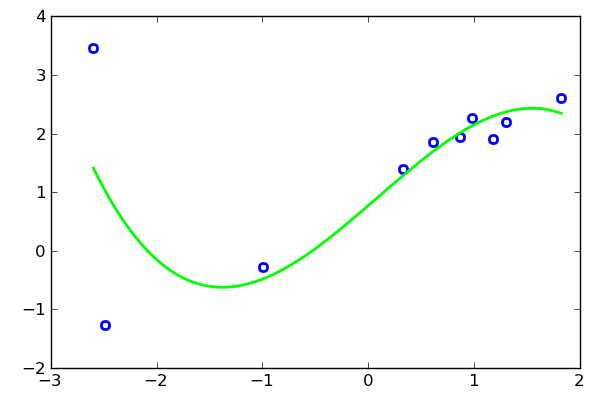
\includegraphics[width = 2.25in]{B-3.png}
	\caption{Training data, $M = 3$, $\lambda = 0.131$}
\end{subfigure} \\

\begin{subfigure}[b]{2.25in}
	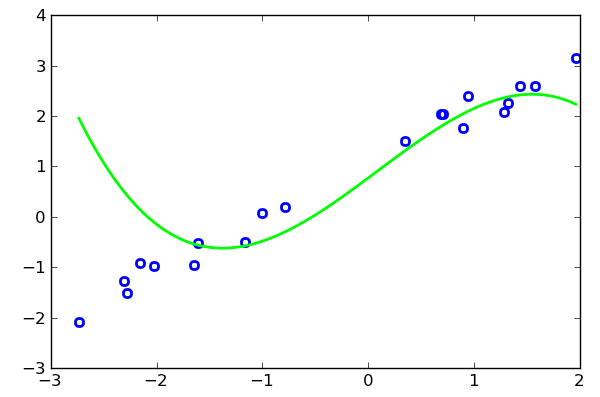
\includegraphics[width = 2.25in]{BV-3.png}
	\caption{Validation data, $M = 3$, $\lambda = 0.131$}
\end{subfigure} \\

\end{tabular}

\caption{The best fit for \textsc{Ridge-Regression} using Regression Data B as training data.}
\end{figure}


\subsection{Applications}

Next, we consider an application of this technique. We will use the BlogFeedback data set, which describes a blog post by 280 numerical values, and maps this to the number of comments the blog post receives in the next 24 hours. We will train our data on one data set and then validate it on another to determine $\lambda$ (here we will use a simple linear model, so $M = 1$). For this data set, we will then apply our curve to a test data set and judge its performance.

Figure 11 shows a plot of the SSE of the validation set versus $\lambda$. We can see that $\lambda$ here is much larger than any value of $\lambda$ we have seen in the past. However, because we are using such a large data set, this is not unreasonable.

\begin{figure}[!]
\centering
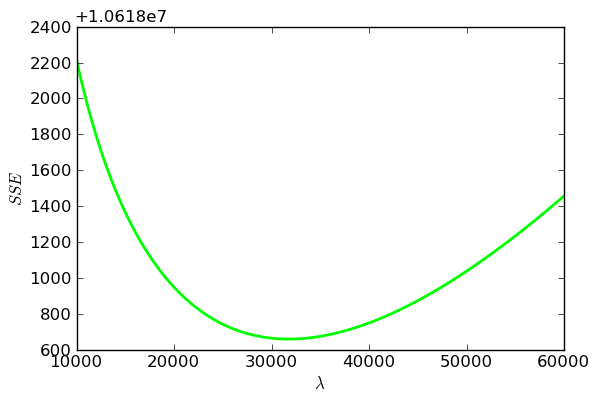
\includegraphics[width=3in]{big_plot.png}
\caption{SSE of the validation data plotted against the value of $\lambda$ used in \textsc{Ridge-Regression} on the BlogFeedback training data. The minimum occurs at $\lambda = 31746$.}
\end{figure}

The minimum of this graph is at $\lambda = 31746$. The SSE of the validation data at this point is $1.062 \cdot 10^7$. Now we have a model for our data. It is interesting to note that the attribute which received the greatest weight in our model is the average number of comments on blog posts from that particular source.

Finally, we check the performance of the model against the test data. We note that the test data and validation data contain the same number of points, so SSE is a reasonable measure to use to compare performance of fit on the test set versus the validation set. Using our model, the SSE for the test set is $9.352 \cdot 10^6$. This is even less than the SSE for the validation data, so our model seems to be a good fit for the data.

\section{Generalizations}


A possible way to avoid having our fit be so perturbed by outliers is to only penalize error linearly instead of quadratically. We repeated our experiments with model fitting using the least absolute deviations fit, where errors are only punished linearly but the regularization term is still quadratic. Because this model does not have a nice closed form solution like ridge regression, we use \textsc{Gradient-Descent} to minimize the sum of the absolute value of the errors plus the quadratic regularization term. Thus, the values in this section are less precise than those in the previous sections.

Figure 12 contains the results for Regression Data A. Note that this time, our goal was not to minimize the SSE of the validation data, but the absolute deviations. Thus, the values in Figure 12 should not be compared to the values in Figure 7. Unsurprisingly, the best fit for the data in this again was $M = 1$ and $\lambda = 0$. The fit produced was extremely similar to that in Figure 8, so we do not show it here. However, this is also unsurprising. Because no point lies very far from our curve, the absolute differences are not very different from the quadratic differences.

\begin{figure}
\centering
\def\arraystretch{1.4}

\newcolumntype{C}[1]{>{\centering\let\newline\\\arraybackslash\hspace{0pt}}m{#1}}

\begin{tabular}{| C{0.75in} | C{0.75in} | C{0.75in} |}

\hline
$M$ & $\lambda$ & AD\\
\hline
1 & 0 & 3.82\\
\hline
2 & 0.2 & 6.34\\
\hline
3 & 1.9 & 9.13\\
\hline
4 & 3.2 & 7.47\\
\hline
5 & 4.1 & 10.60\\
\hline
\end{tabular}
\caption{Optimal values of $\lambda$ when trained on Regression Data A for various values of $M$, along with the resulting AD of the validation data.}
\end{figure}

The more interesting data set here is Regression Data B, which contained a large outlier which caused the quadratic error penalization to behave poorly. Figure 13 shows that results of performing least absolute deviations model fitting on Regression Data B.

\begin{figure}
\centering
\def\arraystretch{1.4}

\newcolumntype{C}[1]{>{\centering\let\newline\\\arraybackslash\hspace{0pt}}m{#1}}

\begin{tabular}{| C{0.75in} | C{0.75in} | C{0.75in} |}

\hline
$M$ & $\lambda$ & AD\\
\hline
1 & 0 & 5.00\\
\hline
2 & 0 & 5.39\\
\hline
3 & 0 & 19.55\\
\hline
4 & 0 & 18.21\\
\hline
5 & 1.4 & 23.20\\
\hline
\end{tabular}
\caption{Optimal values of $\lambda$ when trained on Regression Data B for various values of $M$, along with the resulting AD of the validation data.}
\end{figure}

We can see that the absolute deviation is minimized when $M = 1$ and $\lambda = 0$. Figure 14 shows the resulting curve plotted against Regression Data B and the validation data. We can clearly see that this curve fits the validation data much better than the curve shown in Figure 10.

\begin{figure}[!t]
\centering
\begin{tabular}{c}

\begin{subfigure}[b]{2.25in}
	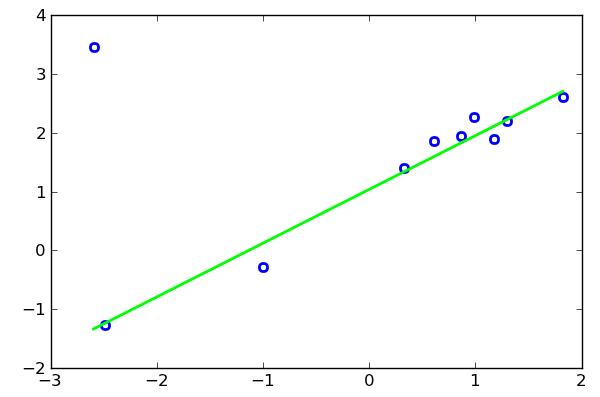
\includegraphics[width = 2.25in]{B-fixed.png}
	\caption{Training data, $M = 1$, $\lambda = 0$}
\end{subfigure} \\

\begin{subfigure}[b]{2.25in}
	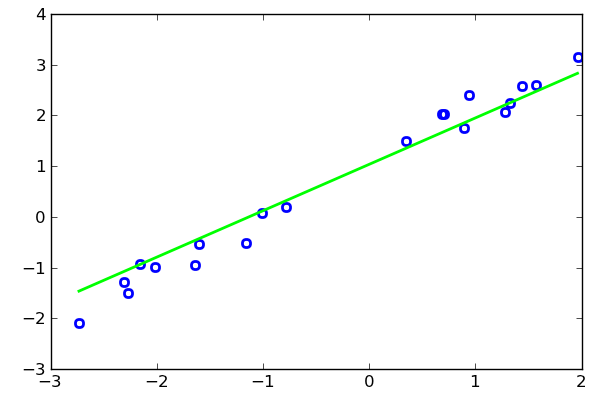
\includegraphics[width = 2.25in]{BV-fixed.png}
	\caption{Validation data, $M = 1$, $\lambda = 0$}
\end{subfigure} \\

\end{tabular}

\caption{The best fit when minimizing LAD using Regression Data B as training data.}
\end{figure}


Another possible fit is to penalize error quadratically, but use a linear regularization term. We used this fit again on Regression Data A and Regression Data B. For Regression Data A, the best parameters were again $M = 1$ and $\lambda = 0$. For Regression Data B, the best parameters were $M = 4$ and $\lambda = 1.2$ (resulting in an SSE of 26.7). Again, because we chose to penalize quadratically for error, the outlier in this data set substantially effects the placement of the curve.


\subsection{Discussion}

The difference in approaches punishing error linearly versus punishing error quadratically is reflected in the different way the two approaches handle outliers. If a data set is expected to have a lot of outliers that do not accurately reflect the future answers, absolute deviations should be used. If a data set is generally clumped, with few misleading outliers, squared deviations should be used, because otherwise some data points might not get as much weight as they deserve. 

The lasso  might be used when there are many features, some of which should be ignored entirely. Linear punishment will push many of the weights all the way to 0, and then the function will be simple to explain, implement, and think about intuitively.

If the prediction problem has absolute value loss, it becomes likelier that absolute differences are the correct choice. The predictor should be trained in such a way as to minimize the loss function that it will suffer when it is used on real data. On the other hand, the amount that high weight vectors should be punished is dependent on the fear of over-fitting; an unusual loss function is unlikely to change the way you punish high weights.

\end{document}